\documentclass[tikz,border=10pt]{standalone}
\begin{document}

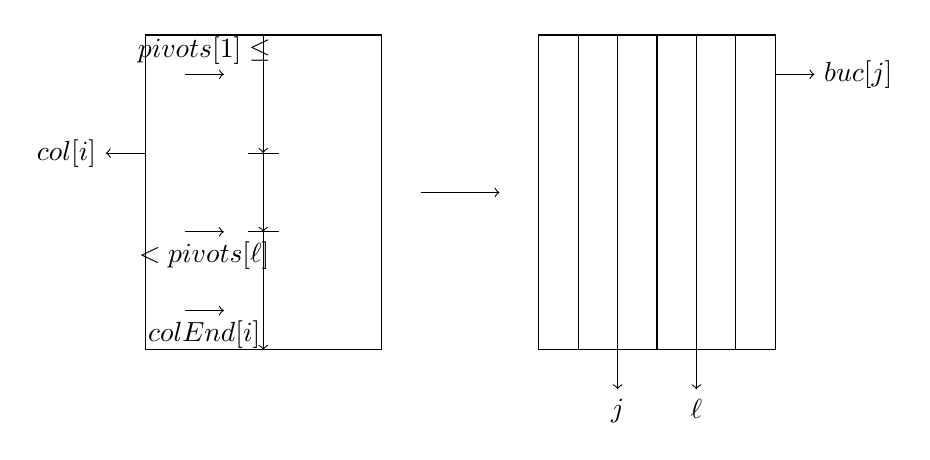
\begin{tikzpicture}

% Left box
\draw (0,0) rectangle (3,4);

% Left box labels
\draw[->] (0.5,3.5) -- (1,3.5) node[midway, above] {$pivots[1] \le$};
\draw[->] (0.5,1.5) -- (1,1.5) node[midway, below] {$< pivots[\ell]$};
\draw[->] (0.5,0.5) -- (1,0.5) node[midway, below] {$colEnd[i]$};

% Left pointer
\draw[->] (0,2.5) -- (-0.5,2.5) node[left] {$col[i]$};

% Left arrows
\draw[->] (1.5,4) -- (1.5,2.5);
\draw[->] (1.5,2.5) -- (1.5,1.5);
\draw[->] (1.5,1.5) -- (1.5,0);

% Left bracket
\draw (1.3,2.5) -- (1.7,2.5);
\draw (1.3,1.5) -- (1.7,1.5);

% Middle arrow
\draw[->] (3.5,2) -- (4.5,2);

% Right box
\draw (5,0) rectangle (8,4);

% Right box columns
\foreach \x in {5.5, 6, 6.5, 7, 7.5} {
    \draw (\x,0) -- (\x,4);
}

% Right box labels
\draw[->] (8,3.5) -- (8.5,3.5) node[right] {$buc[j]$};
\draw[->] (6,0) -- (6,-0.5) node[below] {$j$};
\draw[->] (7,0) -- (7,-0.5) node[below] {$\ell$};

\end{tikzpicture}

\end{document}